In Versuch 241 setzen wir uns mit sogenannten RLC-Schaltungen, also elektrische Schaltungen, welche Widerstände (R), Spulen (L) und Kondensatoren (C) verbinden. In Wissenschaft und Technik haben diese Schaltungen eine vielfältige und weitreichende Menge an Anwendungsfällen. Hierzu gehört zum Beispiel die Erzeugung von Schwingungen in Funktionsgeneratoren, wie sie auch im Praktikum oft zur Anwendung kommen. Die Frequenzabhängigkeit des Wechselstromwiderstandes, der sogenannten Impedanz, kann dazu verwendet werden, um Filterschaltungen zu realisieren. Weiter finden RLC-Glieder in der Signalverarbeitung und Störunterdrückung Anwendung, um beispielsweise Messsignale aufzubereiten und präzisere Messungen zu ermöglichen. Effekte von Widerständen, Induktivitäten und Kapazitäten treten auch in anderen Bauelementen und Kabeln auf. Das Verständnis der Effekte dieser hilft uns, Schaltungen entsprechend zu optimieren, sowie Fehler und Verfälschungen besser Interpretieren zu können.

\subsection{Physikalische Grundlagen}

\subsubsection*{Verhalten eines RC-Gliedes im Zeitbereich}
Zunächst betrachten wir das Verhalten eines RC-Gliedes, also einer Schaltung aus einem Widerstand und einem Kondensator in einer Schaltung mit einer Gleichspannungsquelle, wie in \abbref{fig:schaltpl_rc_ac} dargestellt.

\begin{figure}[H]
  \centering
  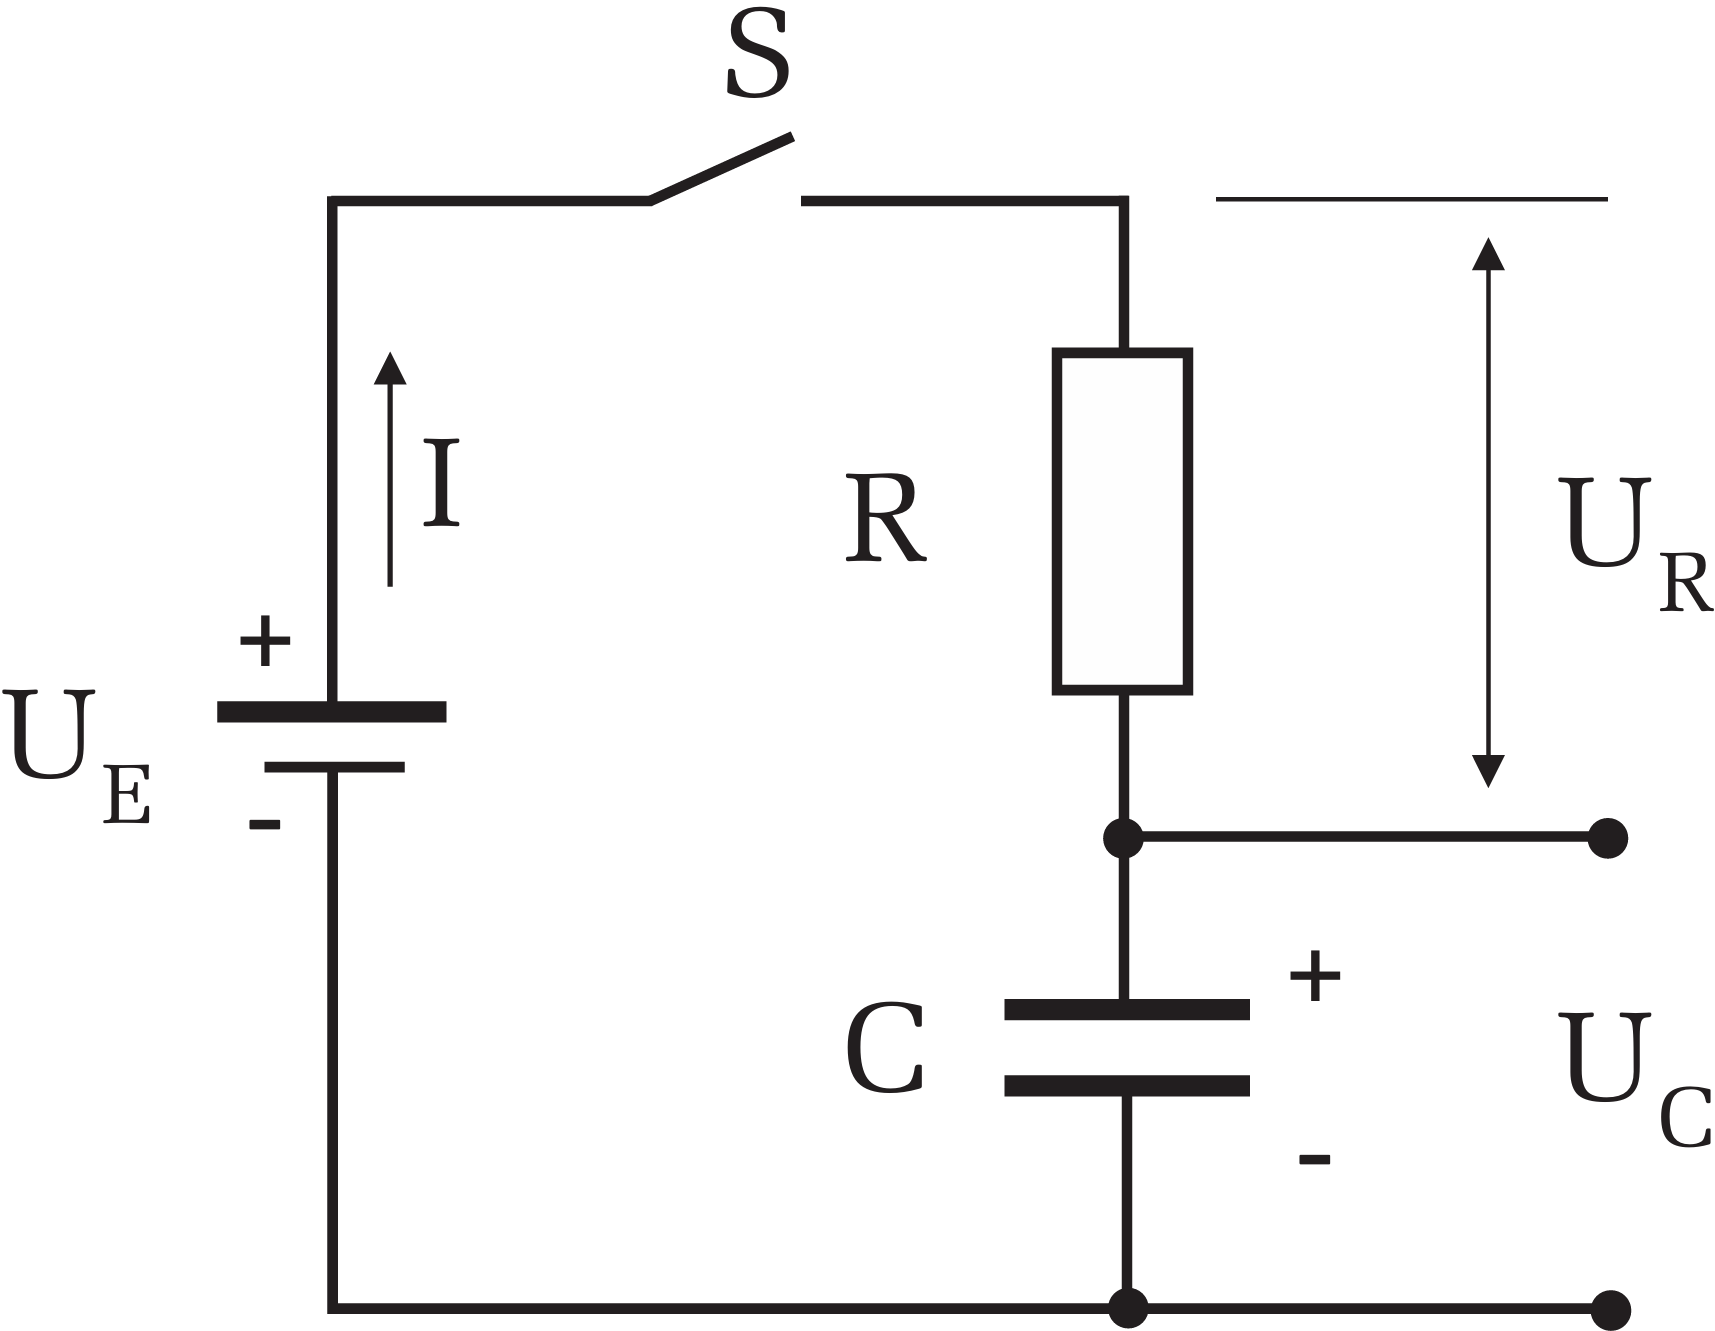
\includegraphics[width=.70\textwidth]{files/script/schaltpl_rc_dc.png}
  \caption{Schaltplan eines RC-Gliedes mit Gleichspannungsquelle}
  \label{fig:schaltpl_rc_ac}
\end{figure}

Wird der Stromkreis geschlossen, so beginnt der Kondensator sich aufzuladen. Der Aufladevorgang ist abschlossen, sobald die Spannung am Kondensator die Eingangsspannung $U_E$ erreicht. Nach der Kirchhoff'schen Maschenregel gilt, dass die Eingangsspannung $U_E$ gleich der Summe der Spannung am Kondensator $U_C$ und am Widerstand $U_R$ entspricht, also
\begin{align}
  U_E = U_C + U_R = U_C + R I.
\end{align}
Der Strom $I$ entspricht gerade der zeitlichen Änderung der Kondensatorladung $I = \dot{Q} = C \dot{U}_C$, wodurch wir die Differentialgleichung
\begin{align}
  U_E = U_C + RC \dot{U}_C
\end{align}
erhalten. Als Lösung dieser Differentialgleichung erhalten wir
\begin{align}
  U_C(t) = U_E\qty(1 - \e{-\flatfrac{t}{\tau}})
\end{align}
Hierbei haben wir mit $\tau = RC$ die Zeitkonstante eingeführt. Erneut nach der Maschenregel können wir aus diesem Ergebnis den Verlauf der Spannung am Widerstand
\begin{align}
  U_R(t) = U_E\e{-\flatfrac{t}{\tau}},
\end{align}
sowie nach dem Ohm'schen Gesetz den Strom
\begin{align}
  I(t) = \frac{U_R(t)}{R} = I_0\e{-\flatfrac{t}{\tau}}
\end{align} 
herleiten. Wir sehen nun, dass die Kondensatorladung exponentiell bis $U_E$ ansteigt, während der Strom von $I_0 = \frac{U_E}{R}$ gegenläufig exponentiell bis $0$ abfällt. Die ausschlagebende größe ist bei diesem Prozess die soeben eingeführte Zeitkonstante $\tau$. Diese lässt sich durch die Messung der Halbwertszeit des $T_{\flatfrac{1}{2}}$ der Kondensatorladung nach 
\begin{align}
  \frac{U_E}{2} &= U_E\qty(1 - \e{\flatfrac{T_{\ffrac{1}{2}}}{\tau}})\\
  \iff \tau &= \frac{\Thalf}{\ln 2}\label{eq:zeitkonst}
\end{align}
bestimmen.

Liegt am RC-Glied eine Rechtecksspannung mit der Periodendauer $T$ an, so wird der Kondensator abwechselnd, abhängig von $\tau$ be- und endladen, wie es in \abbref{fig:spannung_rc_rechteck} dargestellt ist.

\begin{figure}[H]
  \centering
  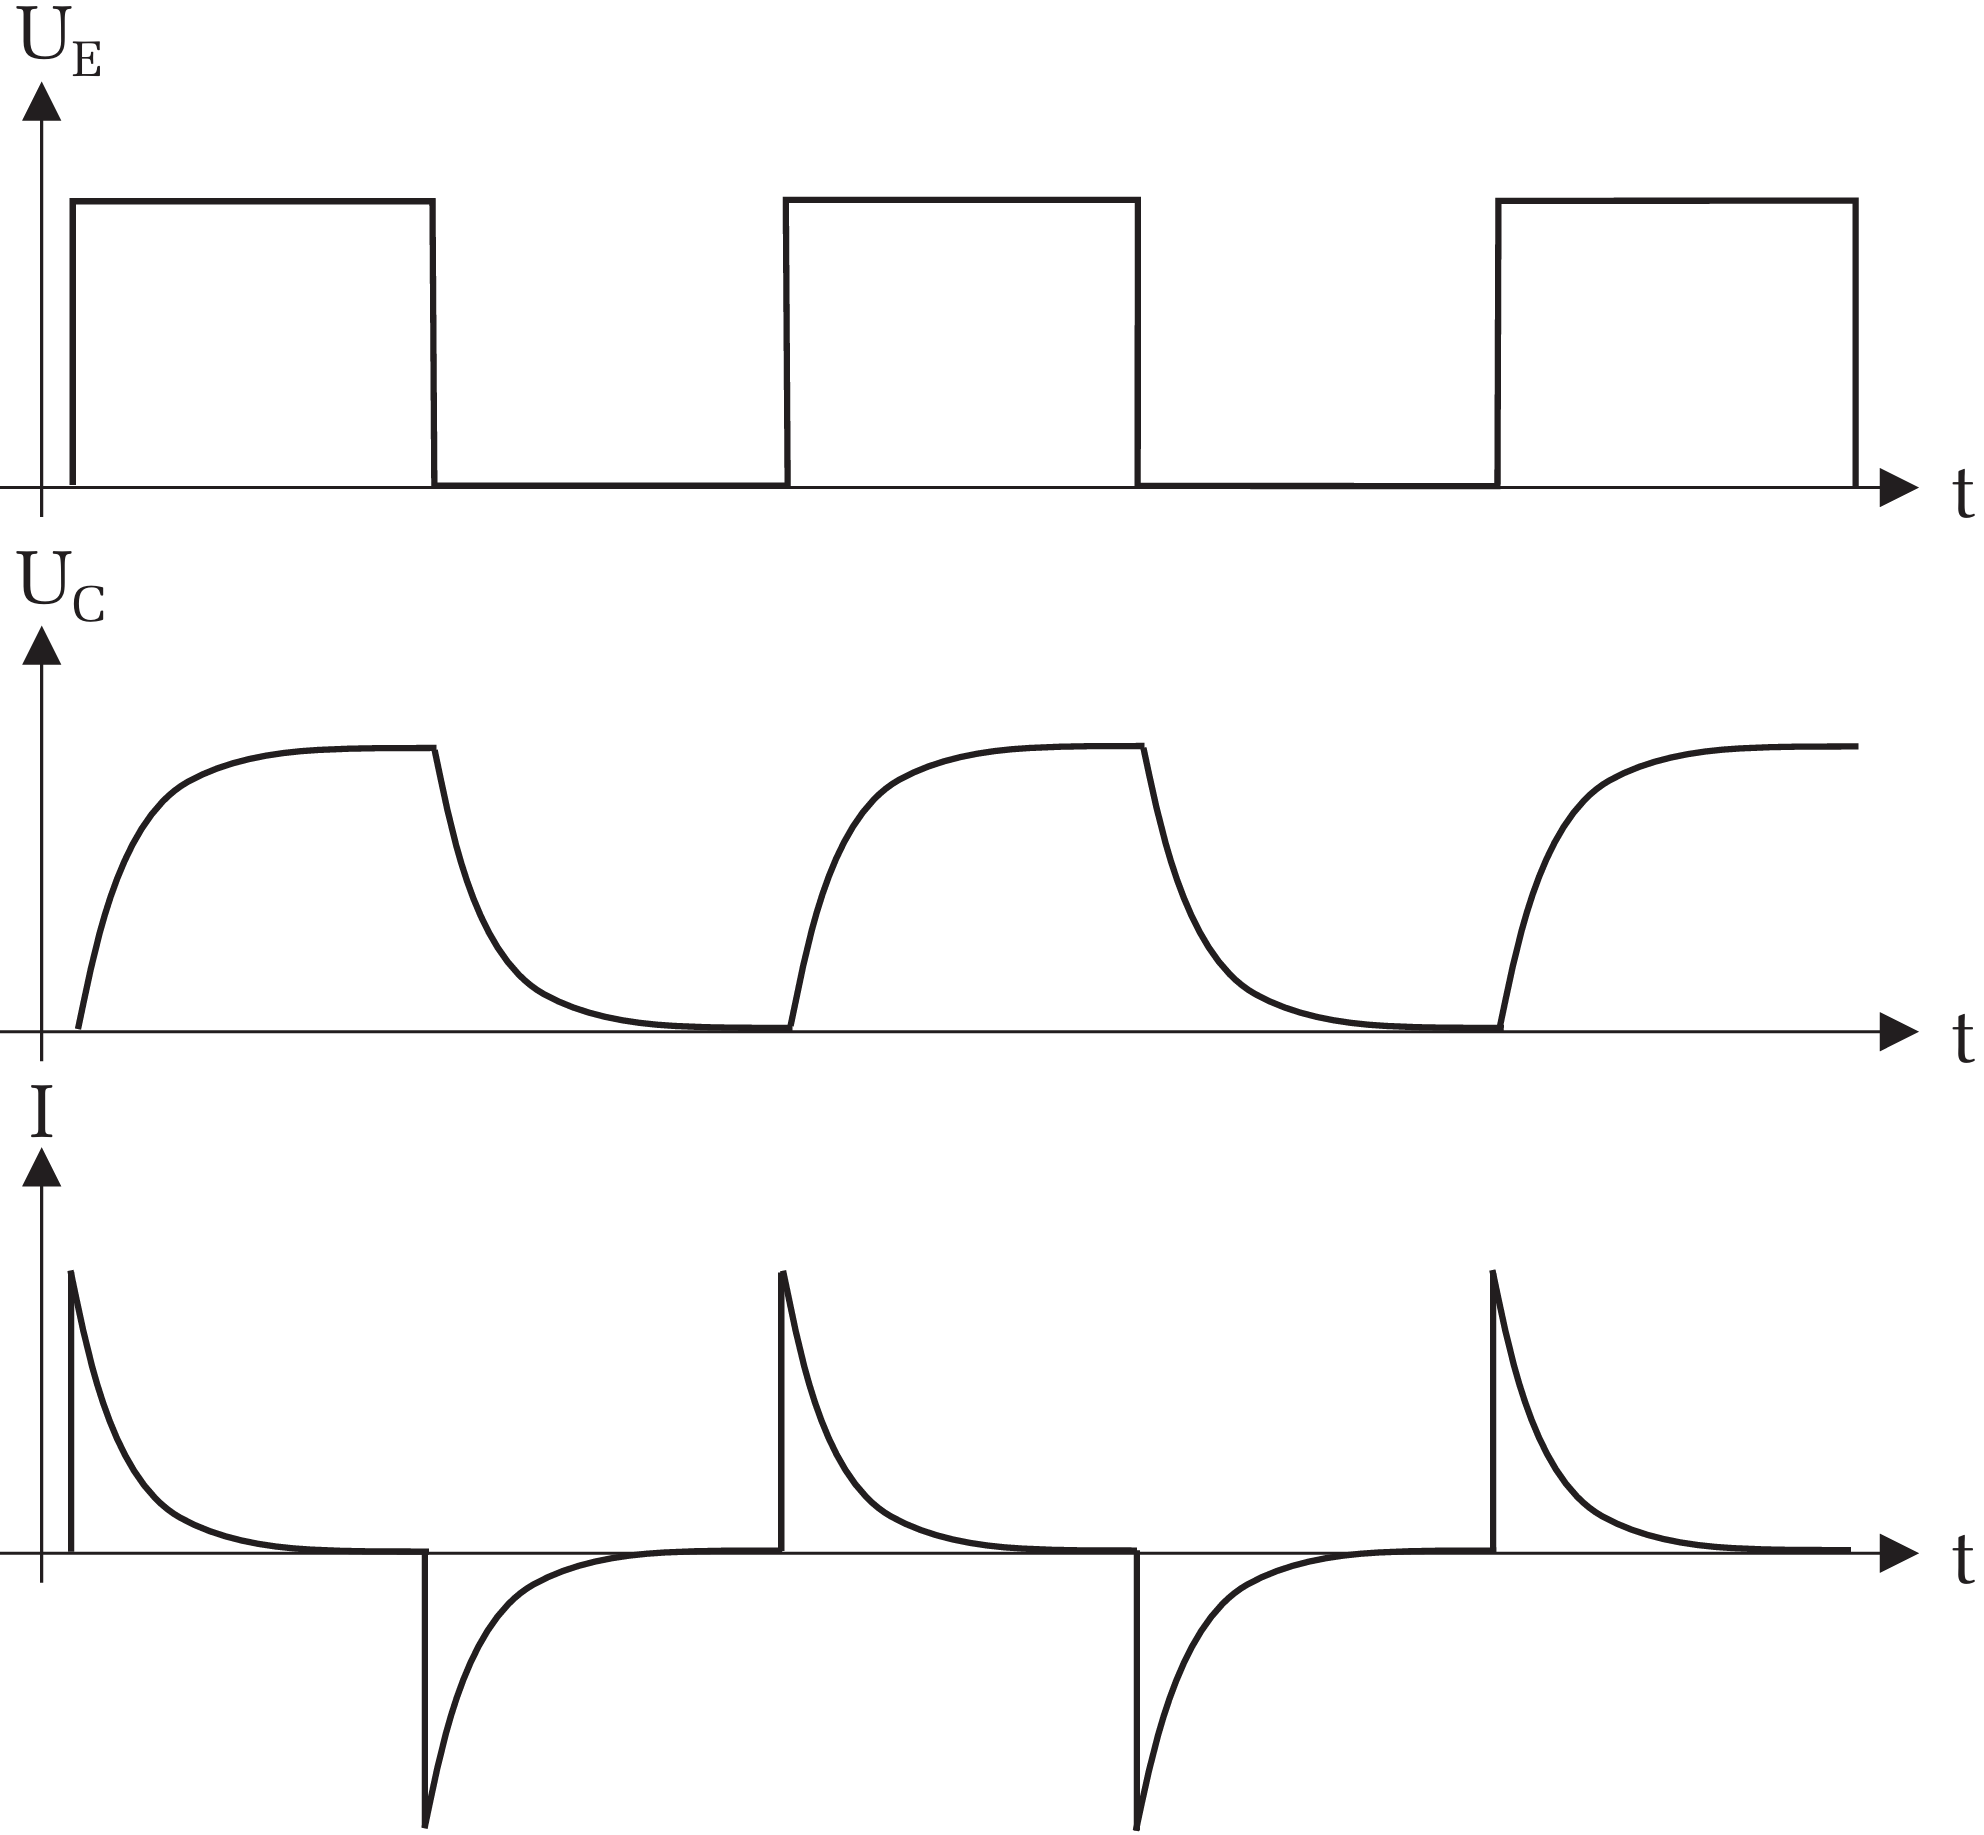
\includegraphics[width=.65\textwidth]{files/script/spannung_rc_rechteck.png}
  \caption{Spannungs- und Stromverlauf am Kondensator im RC-Glied bei eingehendem Rechteckssignal}
  \label{fig:spannung_rc_rechteck}
\end{figure}

\subsubsection*{Impedanz}
Die Impedanz $Z = \ffrac{U}{I}$ bezeichnet den Wechselstromwiderstand, welchen die Bauelemente in einem Wechselstromkreis aufweisen. Die Wechselspannung sei nun beschrieben durch $U_E(t) = U_0\e{i \omega t}$ mit Amplitude $U_0$ und Kreisfrequenz $\omega = 2\pi f$. Für einen ohmschen Widerstand in einem Wechselstromkreis gilt
\begin{align}
  Z_R = \frac{U(t)}{I(t)} = \frac{U_0}{I_0} = R.
\end{align}
Die Impedanz ist also identisch mit dem Gleichstromwiderstand. 

Für einen Kondensator in einem Wechselstromkreis gilt
\begin{align}
  U_E(t) = \frac{Q}{C} \implies \dot{U}_E = \frac{I(t)}{C} \implies i \omega U_E(t) = \frac{I(t)}{C}.
\end{align}
Hierdurch können wir dessen Impedanz herleiten zu
\begin{align}
  Z_C = \frac{U_E(t)}{I(t)} = \frac{1}{i \omega C}.
\end{align}
Eine solche rein imaginäre Impedanz wird auch Blindwiderstand genannt, da dieser Widerstand keine elektrische Leistung verbraucht. Wir stellen außerdem fest, dass die Impedanz frequenzabhängig ist. Für $\omega \to 0$ ist sie unendlich groß, für $\omega \to \infty$ verschwindet sie. Das Auftreten der imaginären Einheit $\frac{1}{i} = \e{-i \frac{\pi}{2}}$ zeigt außerdem eine Phasenverschiebung des Stromes um $-\frac{\pi}{2}$ gegenüber der Spannung auf.

Für eine Spule mit Induktivität $L$ gilt der Zusammenhang
\begin{align}
  U_E(t) &= L \dot{I}(t) = i\omega LI(t)\\[1em]
  \implies Z_E &= i \omega L.
\end{align}
Diese ist also ebenfalls rein imaginär und frequenzabhängig. Auch hier zeigt sich das Auftreten der imaginären Einheit $i = \e{i\frac{\pi}{2}}$ in einer Phasenverschiebung des Stroms um $+\frac{\pi}{2}$ gegenüber der Spannung auf.

\subsubsection*{Frequenzverhalten von RC-Gliedern}

Die soeben festgestellte Frequenzabhängigkeit der Impedanz von Kondensatoren erlaubt es uns, Filterschaltungen zu bauen. Hierzu betrachten wir erneut RC-Glieder, wie sie bereits im ersten Teil zum Einsatz kamen. Wir betrachten eine Schaltung, wie sie in \abbref{fig:schaltpl_rc_ac} dargestellt ist.

\begin{figure}[H]
  \centering
  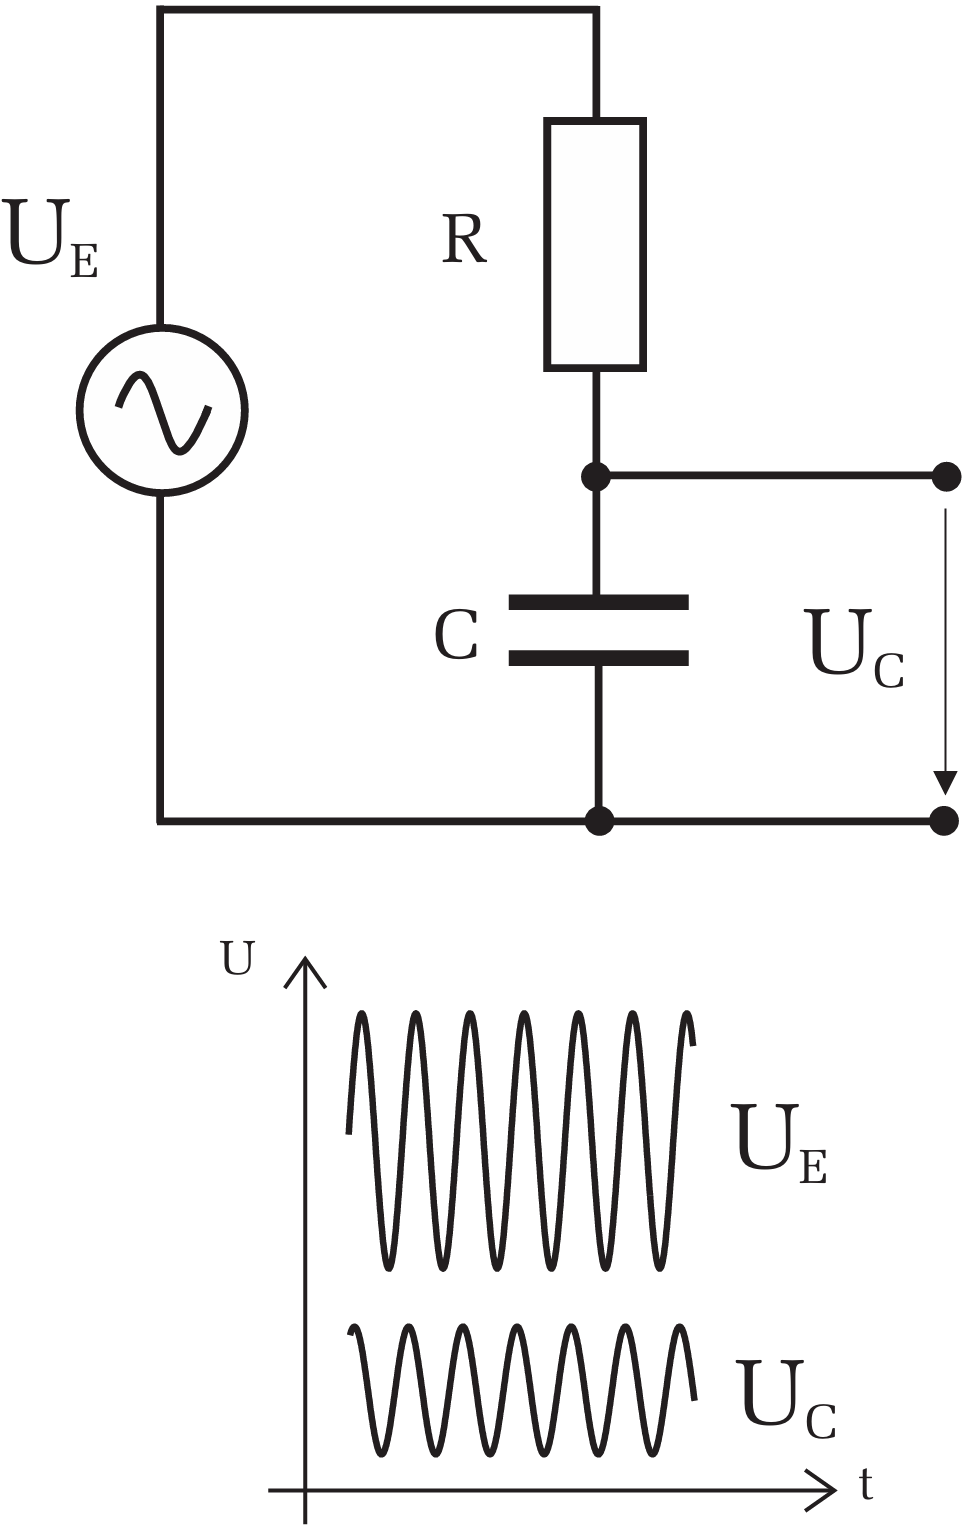
\includegraphics[width=.3\textwidth]{files/script/schaltpl_rc_ac.png}
  \caption{Schaltplan eines RC-Gliedes mit Wechselspannungsquelle}
  \label{fig:schaltpl_rc_ac}
\end{figure}

Die Spannungquelle liefert eine zeitabhängige Wechselspannung, beschrieben durch $U_E(t) = U_0 \e{i\omega t}$. Am Kondensator $C$ nehmen wir eine Spannung ab, für welche nach dem Ohm'schen Gesetz gilt
\begin{align}
  U_C(t) = \frac{Z_C}{R + Z_C} U_E(t).
\end{align}
Hierbei ist $R$ der ohm'sche Widerstand und $Z_C = \frac{-i}{\omega C}$ die komplexe Impedanz des Kondensators. Setzen wir dies in die obere Gleichung ein, so erhalten wir
\begin{align}
  U_C(t) &= \frac{-\ffrac{i}{\omega C}}{R - \ffrac{i}{\omega C}} U_0 \e{i \omega t}\\[1em]
  \intertext{mit dem Betrag}
  \qty|U_C| &= \frac{\qty|U_E|}{\sqrt{1 + (\omega R C)^2}}. \label{eq:ampl_tp}
\end{align}

Am Betrag $\qty|U_C|$ lässt sich erkennen, dass es sich hierbei um einen Tiefpassfilter handelt. Denn, für $\omega \to 0$ geht der Nenner gegen eins und somit $\qty|U_C| \to \qty|U_E|$. Für $\omega \to \infty$ geht auch der Nenner $\to \infty$ und somit $\qty|U_C| \to 0$. Es können also nur niedrige, bzw. tiefe Frequenzen die Schaltung passieren.

Gerade den umgekehrten Effekt erhält man durch Vertauschen des Widerstandes und des Kondensators, wodurch ein Hochpassfilter entsteht. Mit diesem gilt für den Betrag der Spannung am Widerstand
\begin{align}
  \qty|U_R| &= \frac{\qty|U_E|}{\sqrt{1 + \frac{1}{(\omega R C)^2}}}.\label{eq:ampl_hp}
\end{align}

Der Frequenzgang (vergleich \abbref{fig:frequenzgang_tiefpass}) einer solchen Filterschaltung ist definiert als das Verhältnis der Amplituden $\ffrac{\qty|U_A|}{\qty|U_E|}$ über der Frequenz. Die Grenzfrequenz $\omega_g = \frac{1}{RC} = \frac{1}{\tau}$ ist die Frequenz, an welcher die Ausgangsamplitude $\qty|U_A|$ um den Faktor $\frac{1}{\sqrt{2}}$ gegenüber der Eingangsamplitude $\qty|U_E|$ abgefallen (Tiefpassfilter) bzw. angestiegen (Hochpassfilter) ist. Den Bereich bis zur Grenzfrequenz eines Filters nennt man dessen Bandbreite.

\begin{figure}[H]
  \centering
  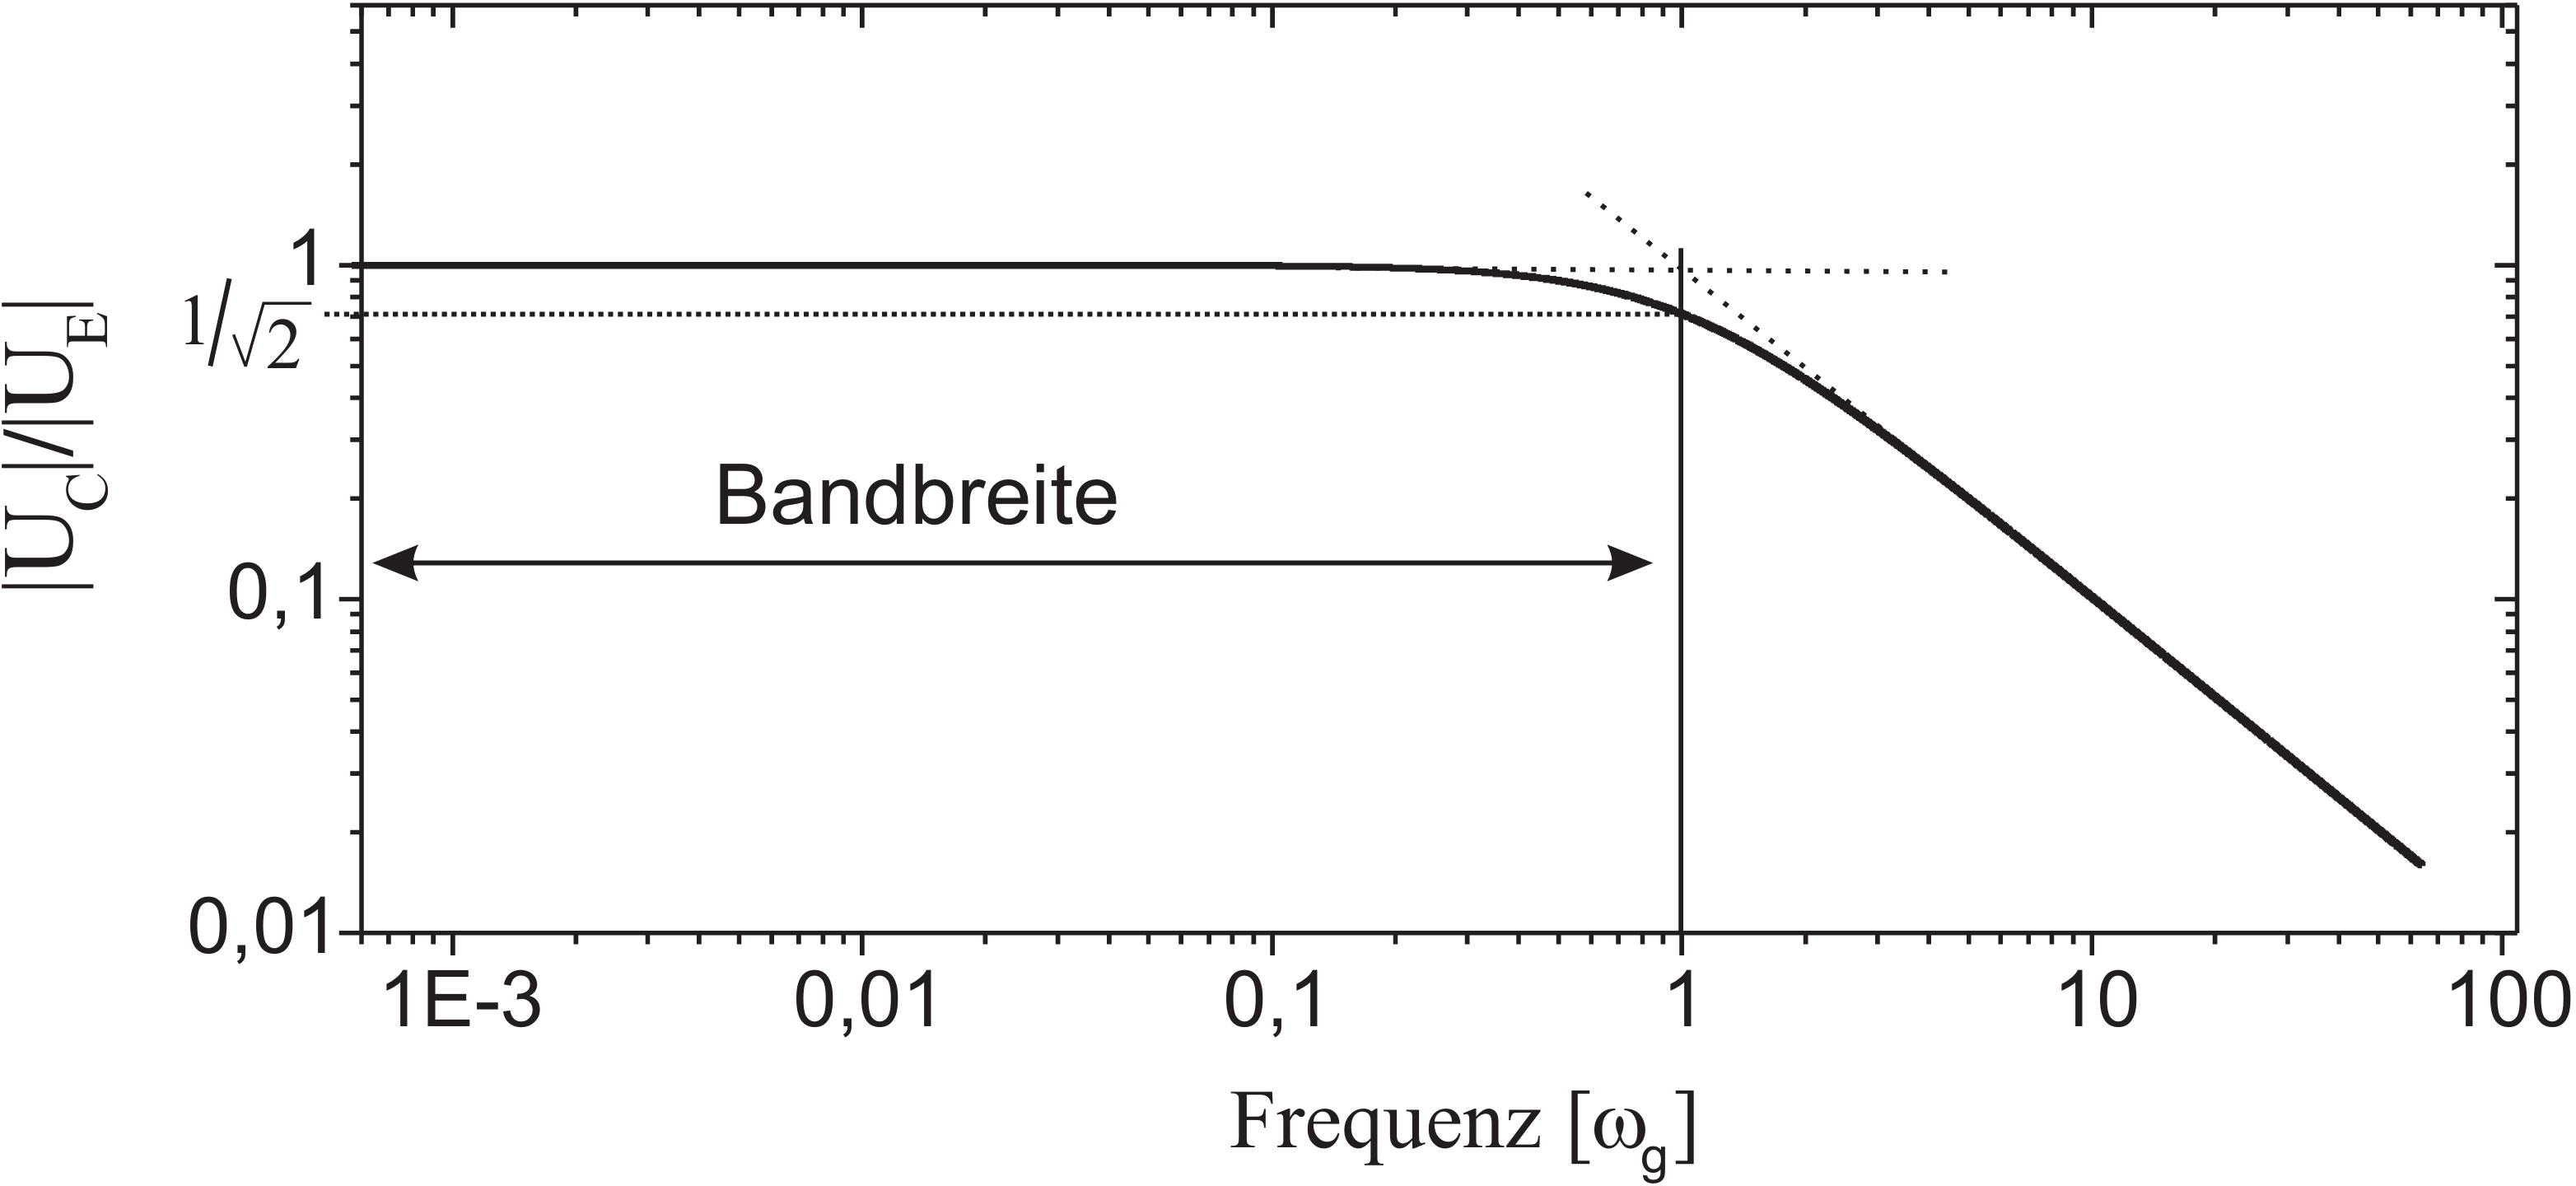
\includegraphics[width=.80\textwidth]{files/script/frequenzgang_tiefpass.png}
  \caption{Frequenzgang eines Tiefpassfilters}
  \label{fig:frequenzgang_tiefpass}
\end{figure}

\subsubsection*{RC-Glied als Differenzier- und Integrierglied}

Ein weiterer Anwendungsbereich von Hoch- und Tiefpassfilterschaltungen ist die Anwendung als Differenzier- und Integrierglieder. Betrachten wir zunächst einen Tiefpassfilter. Der Strom $I$ ergibt sich sowohl anhand der zeitlichen Änderung der Kondensatorladung, also auch dem ohm'schen Gesetz, nach
\begin{align}
  I = C \dv{U_A}{t} = \frac{U_E - U_A}{R}.
\end{align}
Ist nun die Periodendauer $T$ der Eingangsspannung $U_E$ deutlich kleiner als die Zeitkonstante $\tau$, so ist nach \eqref{eq:ampl_tp} $U_A \ll U_E$ und es ergibt sich die Näherung
\begin{align}
  \dv{U_A}{t} &\approx \frac{U_E}{RC}.
  \intertext{Somit entspricht das Ausgangssignal des Tiefpassfilters}
  U_A &\approx \frac{1}{RC} \int U_E \dd{t}.
\end{align}
für die Bedingung $\tau \gg T$ ungefähr dem Integral des Eingangssignals.

Wiederum umgekehrt betrachten wir nun für einen Hochpassfilter die Summe der Teilspannungen. Die Eingangsspannung entspricht der Summe der Spannung am Kondensator
\begin{align}
  U_C = \frac{Q}{C} = \frac{1}{C} \int I \dd{t}
\end{align}
und der Spannung am Widerstand, also der Ausgangsspannung $U_A$. Für dem Strom gilt somit
\begin{align}
  \int I \dd{t} &= C(U_E - U_A) \implies I = C \dv{t} (U_E - U_A).
\end{align}
Unter der Annahme, dass $\tau \ll T$ ist nach \eqref{eq:ampl_hp} $U_A \ll U_E$. Es gilt somit
\begin{align}
  I &\approx C \dv{t}U_E,
  \intertext{also}
  IR = U_A &\approx RC \dv{t} U_E.
\end{align}
Das Ausgangssignal des Hochpassfilters stellt also unter der Bedingung, dass $\tau \ll T$ ist, ungefähr die Differentation des Eingangssignals dar.

\subsubsection*{Elektrischer Schwingkreis (RLC-Glied)}

Wir betrachten zunächst einen idealisierten Schaltkreis mit einem Kondensator und einer parallel geschalteten Spule. Entlädt sich der Kondensator, so wird durch den Entladestrom ein Magnetfeld in der Spule erzeugt. Die im Kondensator gespeicherte elektrische Energie wird also allmählich in magnetische Energie umgewandelt. Sobald der Kondensator gänzlich entladen ist, beginnt der Strom abzunehmen und als Konsequenz des Induktionsgesetzes und der Lenz'schen Regel wird in der Spule ein entgegengesetzter Strom erzeugt. Dieser lädt den Kondensator mit umgekehrter Polung wieder auf, die magnetische Energie wird also wieder in elektrische Energie umgewandelt. Dieses wechselwirkende Verhalten gibt den Schwingkreisen ihren Namen. In der Realität sorgen Widerstände in den Bauteilen, sowie dielektrische wie magnetische Verluste dafür, dass die Schwingung nicht ewig anhält, sondern gedämpft ist, soweit sie nicht durch ein kontinuierliches Eingangssignal angeregt ist. Daher betrachten wir nun RLC-Glieder, welche neben der Spule (L) und dem Kondensator (C) auch einen Widerstand (R) enthalten.

In einem RLC-Serienschwingkreis sind die drei Bauteile in Reihe geschaltet. Die Einzelspannungen, die an den einzelnen Bauteilen abfallen sind
\begin{align}
  U_R = \frac{R}{I}, \quad U_C = \frac{Q}{C}, \quad U_L = -L\dv{t}I.
\end{align}
Nach der Kirchhoff'schen Maschenregel gilt weiter
\begin{align}
  U_R + U_C - U_L = 0,
\end{align}
die Summe der Teilspannungen muss also verschwinden. Durch Einsetzen und differenzieren erhalten wir hieraus die folgende Gleichung
\begin{align}
  L \dv[2]{t} I + R \dv{t} I + \frac{1}{C} I = 0.
\end{align}
Dies entspricht der allgemeinen Differentialgleichung für den gedämpften harmonischen Oszillator. Unter der Annahme, dass der Widerstand verschwindet erhalten wir die Differentialgleichung
\begin{align}
  \dv[2]{t} I + \omega_0 I = 0
\end{align}
eines ungedämpften harmonischen Oszillators mit der Lösung
\begin{align}
  I = I_0 \e{i(\omega_0 t + \varphi)}.
\end{align}
Hierbei wurden Induktivität und Kapazität zur Eigenfrequenz, definiert durch die Thomson'sche Schwingungsformel,
\begin{align}
  \omega_0 = \frac{1}{\sqrt{LC}}
\end{align}
zusammengefasst.

Die allgemeine Lösung des gedämpften harmonischen Oszillators ist gegeben durch
\begin{align}
  I(t) = I_0 e^{-\frac{R}{2L} t} \qty( c_1 e^{\sqrt{\frac{R^2}{4L^2} - \frac{1}{LC}} t} + c_2 e^{-\sqrt{\frac{R^2}{4L^2} - \frac{1}{LC}} t}).
\end{align}
Die Konstanten $c_1$ und $c_2$ hängen dabei von den Anfangsbedingungen ab. Unter der Voraussetzung
\begin{align}
  \frac{R^2}{4L^2} < \frac{1}{LC},
\end{align}
also einer entsprechend schwachen Dämpfung, spricht man vom sogenannten \textit{Schwingfall}. Nur in diesem Fall kommt es auch tatsächlich zu einer periodischen, exponentiell gedämpften Oszillation des Stroms nach
\begin{align}
  I &= I_0 \e{-\frac{R}{2L} t} \e{i(\omega_f t + \varphi)}
  \intertext{mit}
  \omega_f &= \sqrt{\frac{1}{LC} - \frac{R^2}{4 L^2}}.
\end{align}

Wie aus dem Term abzulesen ist, nimmt die Amplitude proportional zu $\e{-\delta t}$ ab. Hierbei ist die Dämpfungskonstante $\delta$ definiert als
\begin{align}
  \delta = \frac{R}{2L}.
\end{align}
Ihr Kehrwert $\ffrac{1}{\delta}$ ist die Relaxationszeit oder Abklingzeit $\tau_r$. Empirisch kann die Dämpfungskonstante durch das Vermessen der Amplituden und der Periodendauer bestimmt werden. Das logarithmische Dekrement
\begin{align}
  \Lambda = \ln(\frac{A_n}{A_{n+1}}) = \delta T\label{eq:log_dekr}
\end{align}
stellt den zugehörigen mathematischen Zusammenhang her.

\subsubsection*{Frequenzabhängigkeit eines Schwingkreises - Resonanz}

Wird ein Schwingkreis durch ein extern anliegendes Sinussignal angeregt, oszilliert dieser mit derselben Frequenz wie das angelegte Signal. Wie bereits im Abschnitt zu Impedanzen betrachtet, hängt jedoch die Amplitude des Ausgangssignals von der eingehenden Frequenz ab. Für die Gesamtimpedanz $Z_g$ in einem Serienschwingkreis gilt
\begin{align}
  Z_g = Z_R + Z_C + Z_L = R + i\qty(\omega L - \frac{1}{\omega C}).
\end{align}
Hieraus folgt für den Strom im Schwingkreis nach dem ohm'schen Gesetz
\begin{align}
  I = \frac{U_E}{Z_g} = \frac{1}{R + i\qty(\omega L - \frac{1}{\omega C})} U_0 \e{i(\omega t - \varphi)},
\end{align}
wobei $U_E(t) = U_0 \e{i(\omega t)}$ das Eingangssignal darstellt. Dessen Betrag
\begin{align}
  I_0(\omega) = \frac{U_0}{\sqrt{(R^2 + \qty(\omega L - \frac{1}{\omega C}))^2}}
\end{align}
ist abhängig von der Anregungsfrequenz $\omega$ und nimmt bei der Resonanzfrequenz $\omega_R$
\begin{align}
  \omega_R = \sqrt{\frac{1}{LC}}\label{eq:rlc_omega_r}
\end{align}
das Maximum von $I_0(\omega_R) = \ffrac{U_0}{R}$ an. Es wirkt im Resonanzfall nur der ohm'sche Widerstand, die Schaltung stellt hier also einen Kurzschluss dar. Für die Phasenverschiebung gilt
\begin{align}
  \tan \varphi = \frac{\omega L - \ffrac{1}{(\omega C)}}{R},
\end{align}
im Resonanzfall sind Strom und Spannung also in Phase.

Für die Amplituden der Spannungen an den einzelnen Bauteilen gelten die Zusammenhänge
\begin{align}
\qty| U_R | = \frac{R}{\qty( R^2 + \qty( \omega L - \frac{1}{\omega C} )^2 )^{\ffrac{1}{2}}} U_0,\\
\qty| U_C | = \frac{1/(\omega C)}{\qty( R^2 + \qty( \omega L - \frac{1}{\omega C} )^2 )^{\ffrac{1}{2}}} U_0,\\
\qty| U_L | = \frac{\omega L}{\qty( R^2 + \qty( \omega L - \frac{1}{\omega C} )^2 )^{\ffrac{1}{2}}} U_0.
\end{align}

Betrachten wir die Amplitude $\qty| U_R |$ der Spannung am Widerstand so zeigt sich für verschiedene Werte des Widerstandes das in \abbref{fig:resonanzkurve_widerstaende} abgebildete Verhalten. 

\begin{figure}[H]
  \centering
  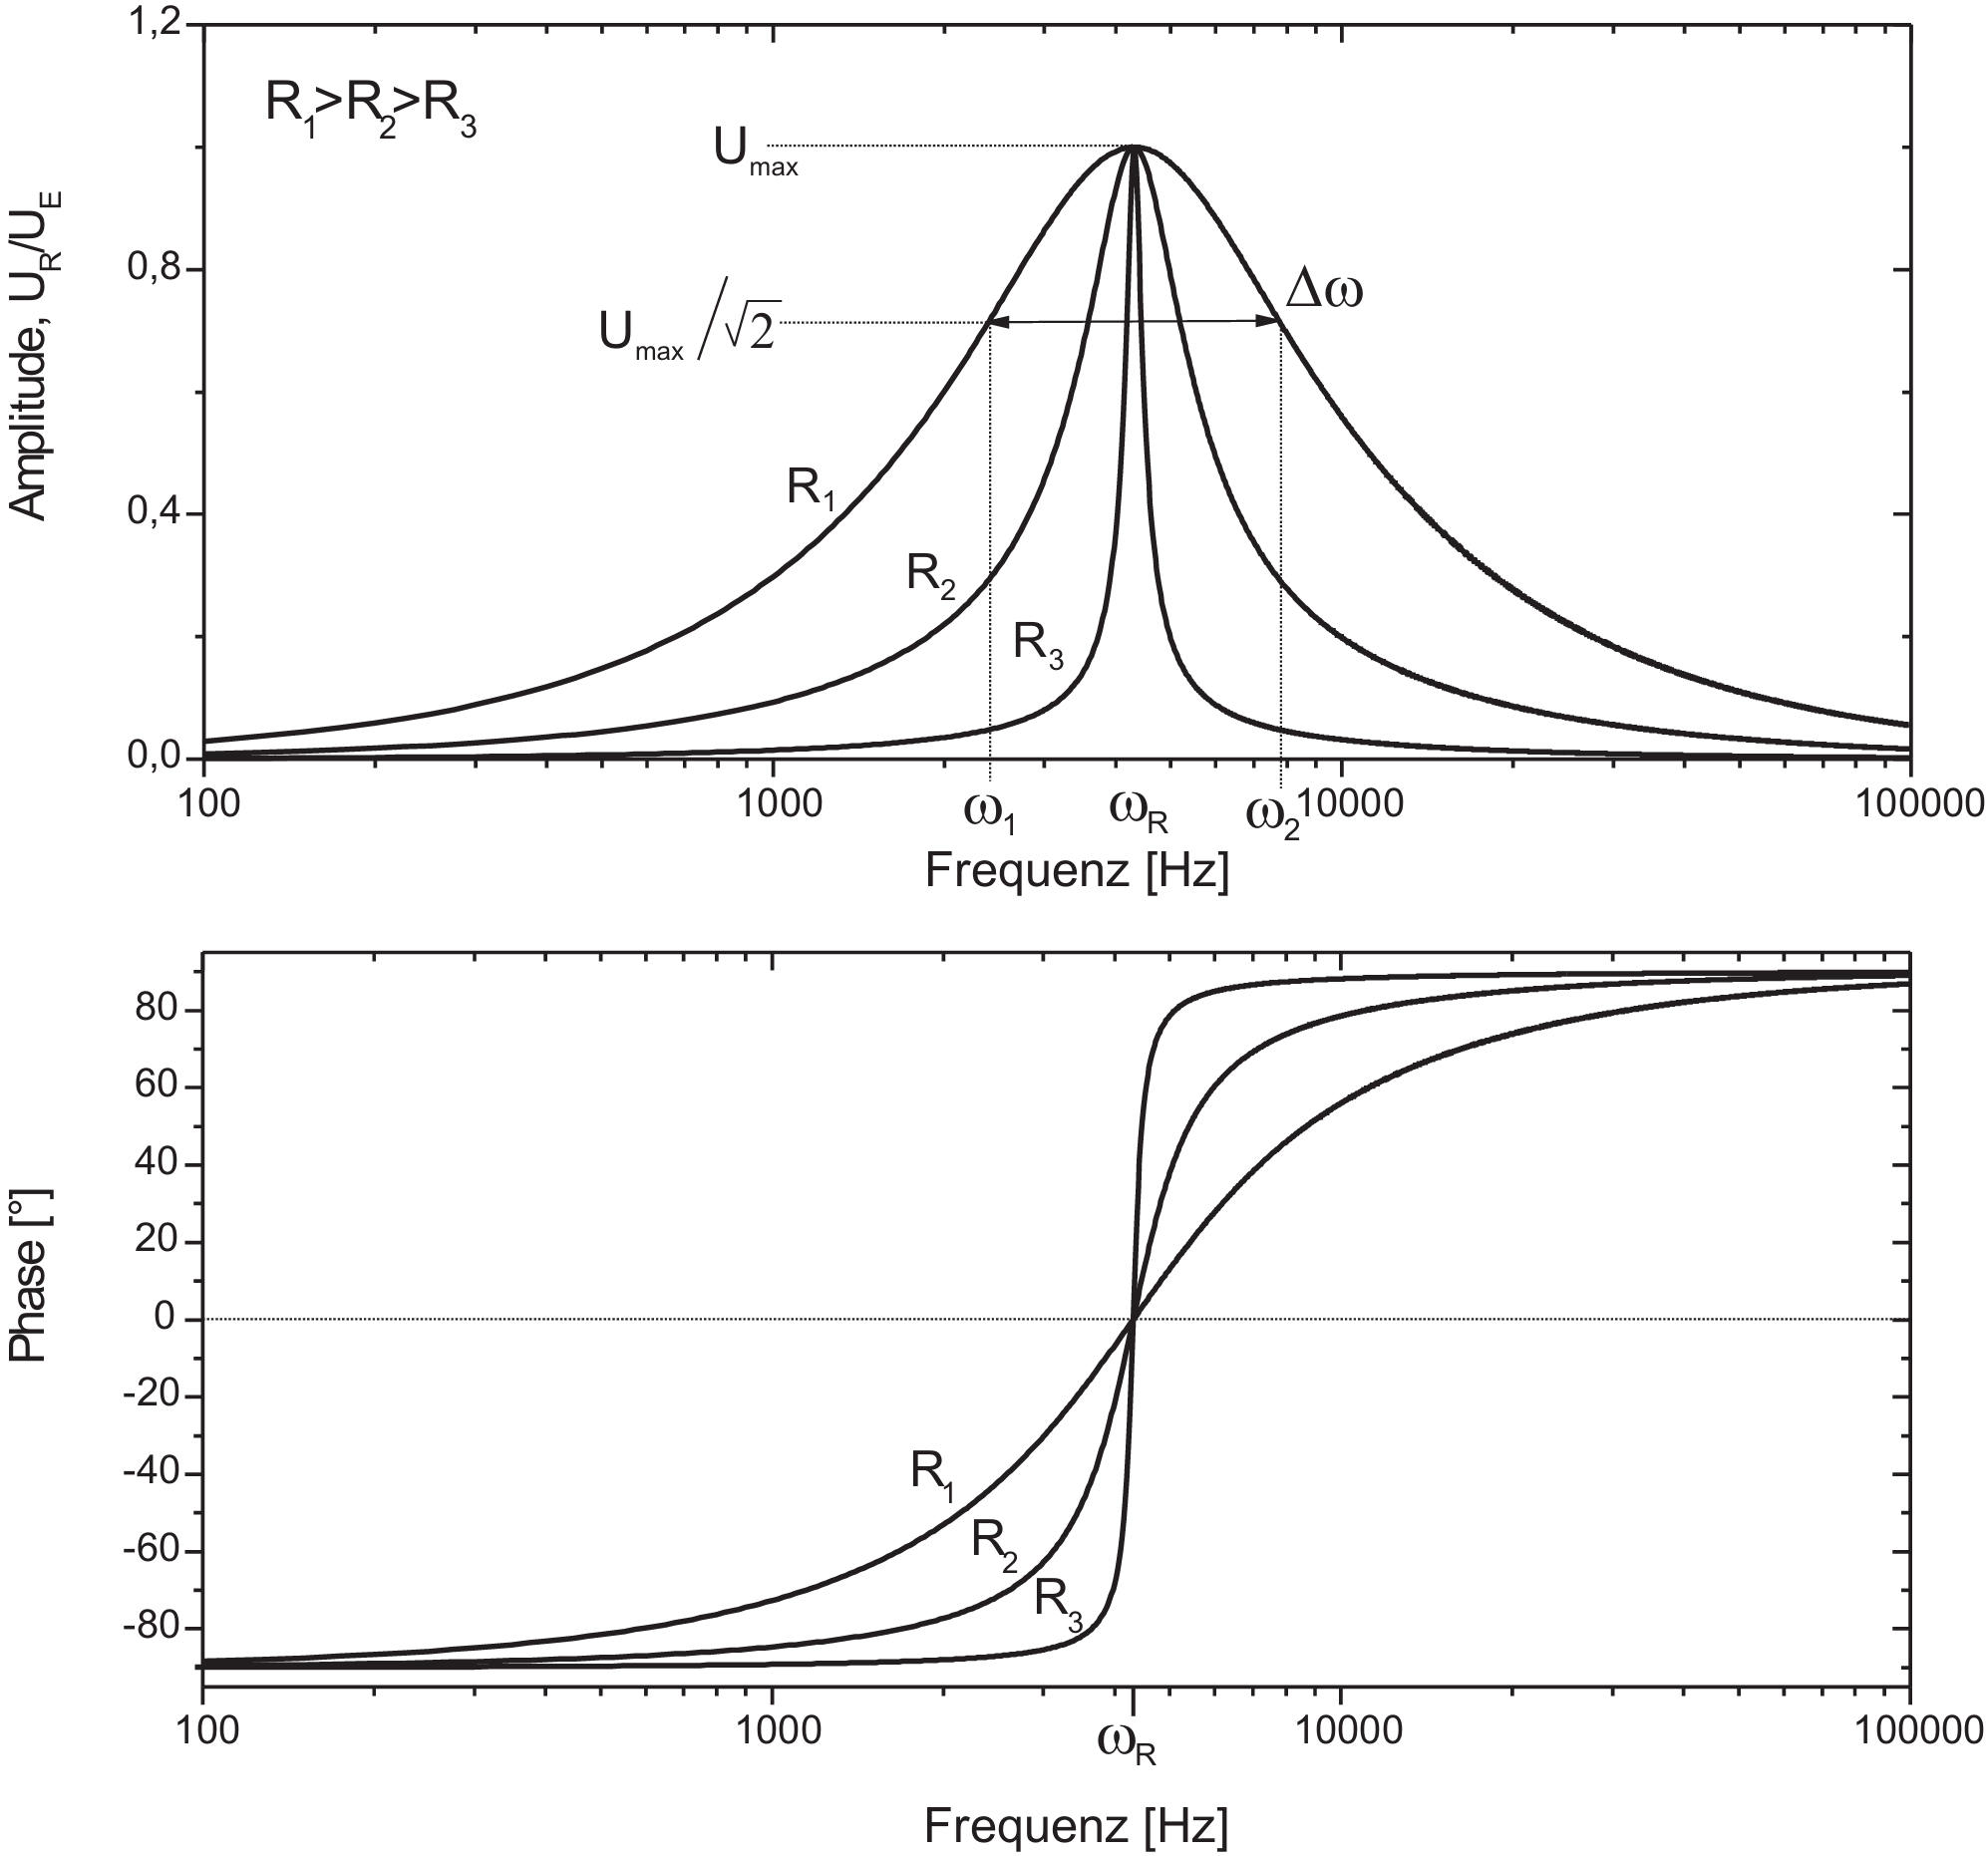
\includegraphics[width=.70\textwidth]{files/script/resonanzkurve_widerstaende.png}
  \caption{Resonanzkurven im RLC-Schwingkreis für verschiedene Werte des Widerstands}
  \label{fig:resonanzkurve_widerstaende}
\end{figure}

Da, wie soeben gezeigt, im Resonanzfall die Gesamtimpedanz von Spule und Kondensator verschwindet, fällt die gesamte Eingangsspannung am Widerstand ab. Die Ausgangsamplitude hier in etwa der Eingangsamplitude. Für von der Resonanzfrequenz abweichende Frequenzen, werden Spule und Kondensator nicht kurzgeschlossen, es fällt also ein teil der Spannung auch an diesen Bauteilen ab. Nach diesem Wirkungsprinzip stellt der Serienschwingkreis einen Bandpass-Filter dar, welcher nur ein bestimmtes Frequenzband um die Resonanzfrequenz passieren lässt. Die Bandbreite ist hier, ähnlich zum Hoch- und Tiefpassfilter, durch die Frequenzen definiert, bei welchen die Amplitude auf das $\sqrt{2}$-Fache gedämpft wird:
\begin{align}
  \Delta \omega = \omega_1 - \omega_2 = \frac{R}{L} = 2\delta.\label{eq:rlc_bandbreite}
\end{align}

\begin{figure}[H]
  \centering
  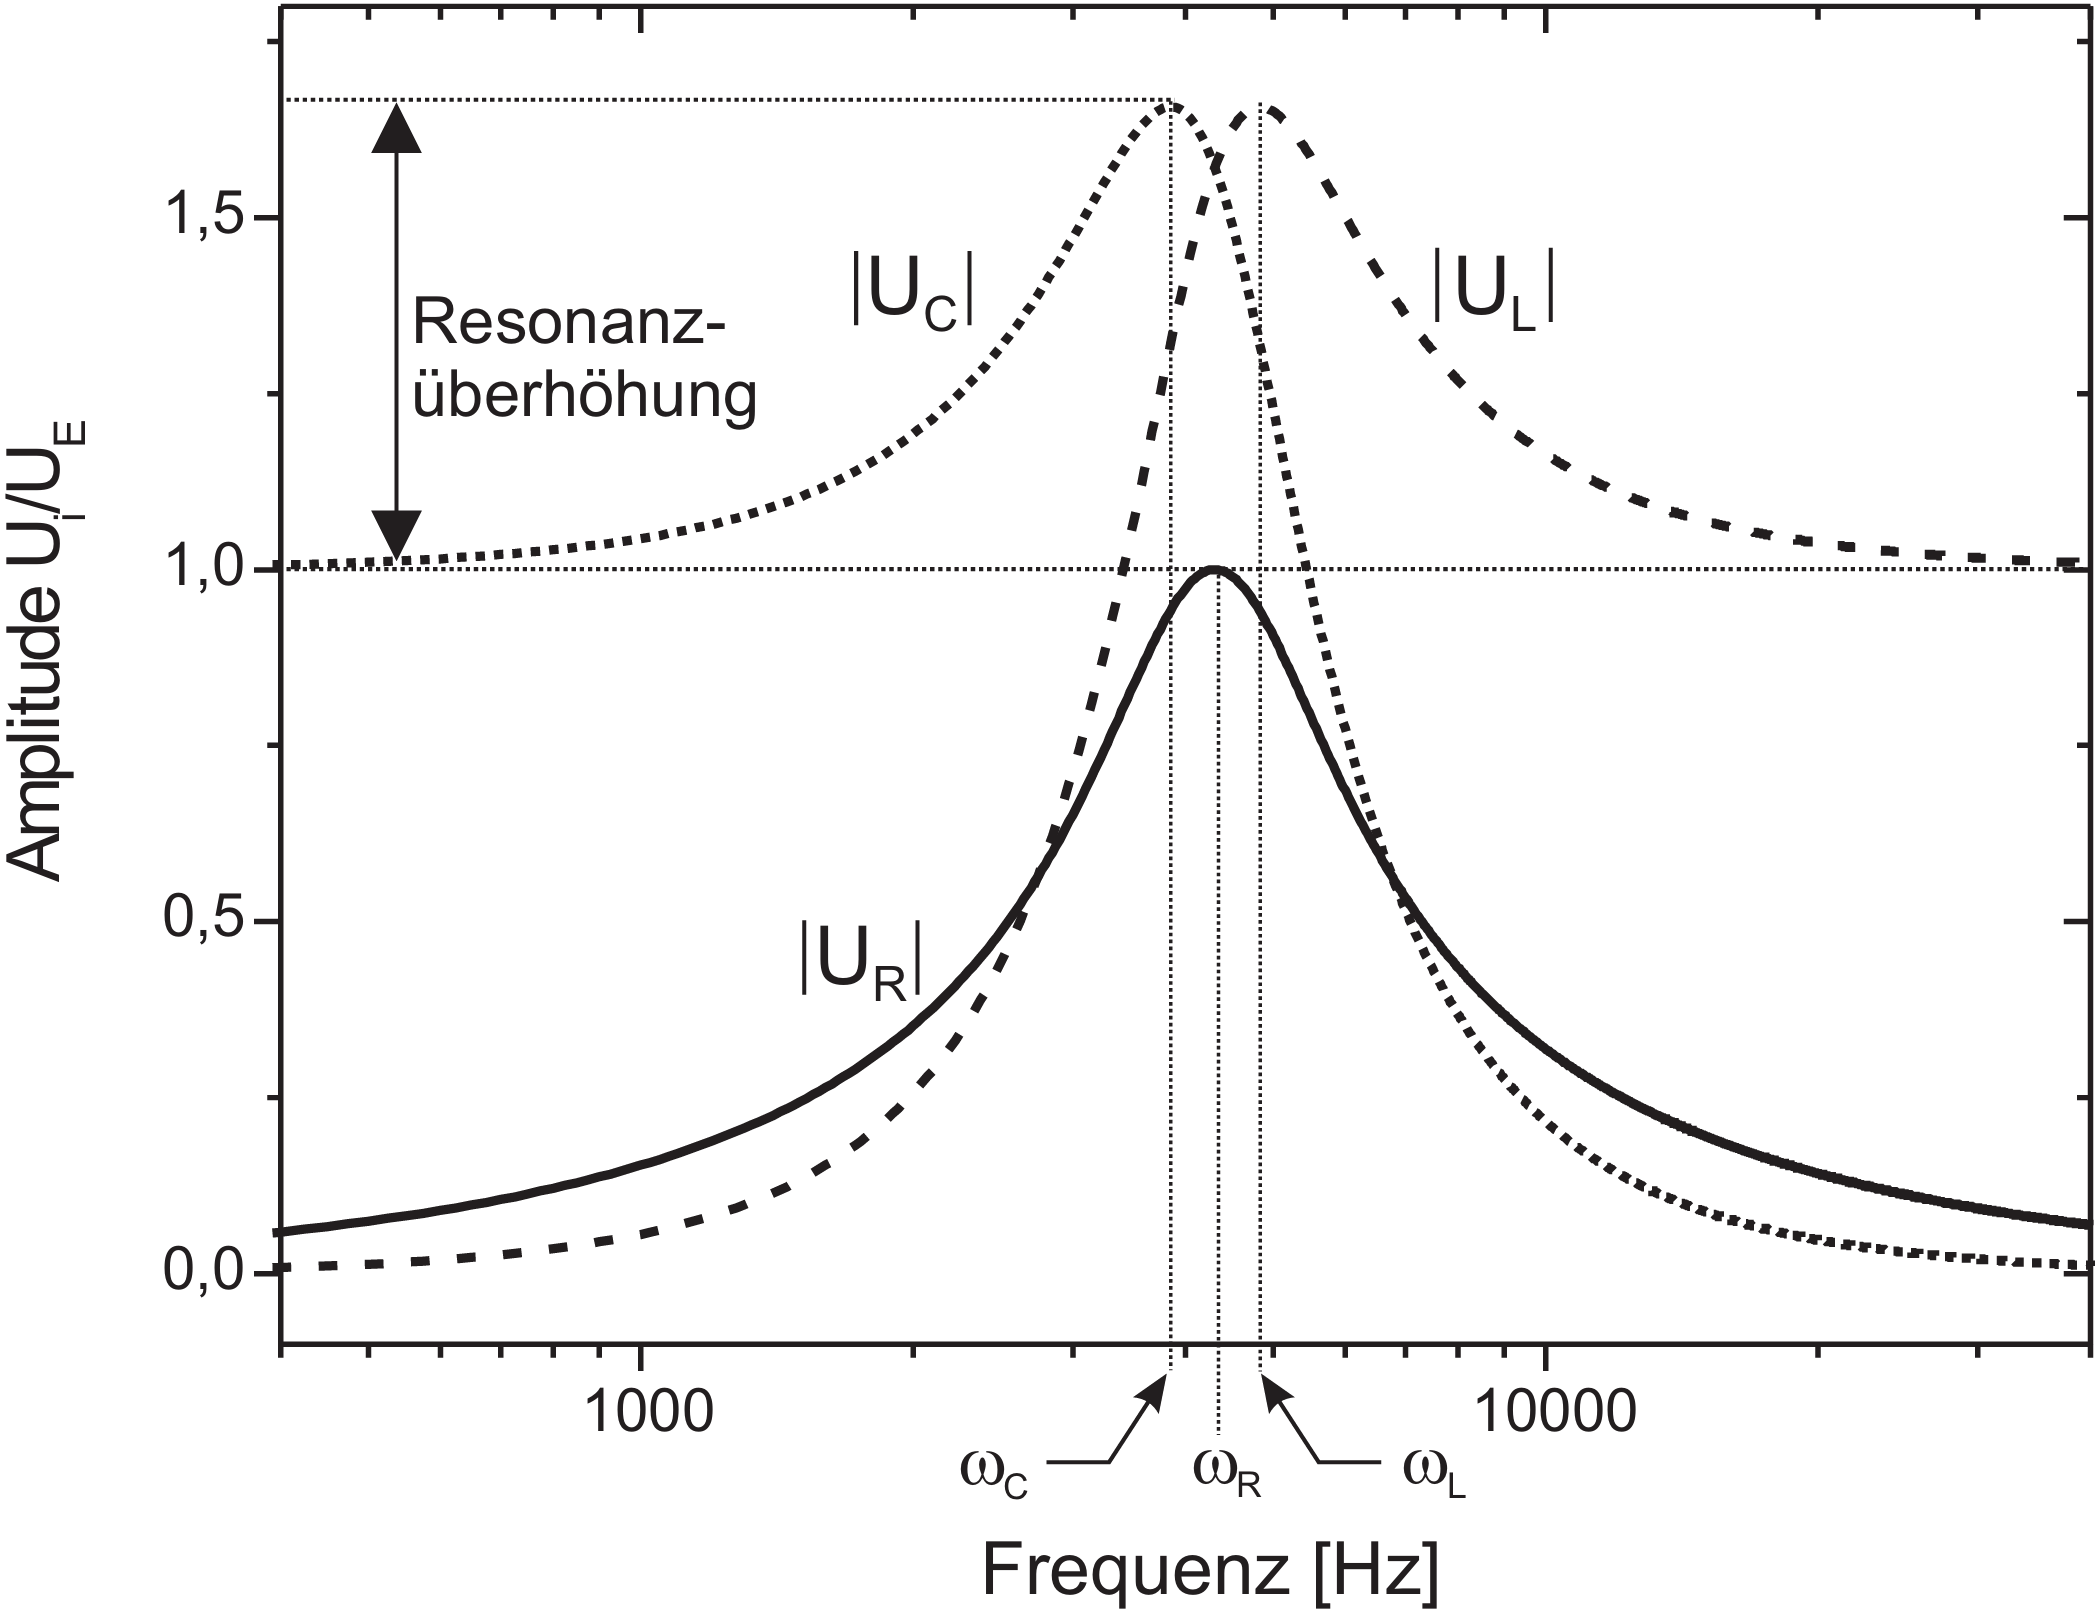
\includegraphics[width=.70\textwidth]{files/script/resonanzkurve_rlc.png}
  \caption{Resonanzkurven im RLC-Schwingkreis, abgenommen an den drei verschiedenen Bauteilen}
  \label{fig:resonanzkurve_rlc}
\end{figure}

\abbref{fig:resonanzkurve_rlc} zeigt nun die Amplituden der Spannungen an allen drei Bauteilen. Zunächst fällt auf, dass die Resonanzfrequenzen für Spule ($\omega_L$) und Kondensator ($\omega_C$) nach rechts bzw. links zur Resonanzfrequenz des Widerstandes verschoben sind. Für diese gilt
\begin{align}
  \omega_C &= \sqrt{\omega_R^2 - 2\delta^2},\label{eq:rlc_omega_c}\\
  \omega_L &= \sqrt{\omega_R^2 + 2\delta^2}.\label{eq:rlc_omega_l}
\end{align}

Weiter fällt auf, dass hier die Ausgangsamplituden über den Wert der Eingangsamplitude hinaus steigen. Diese sogenannte Resonanzüberhöhung kommt ohne verstärkendes Bauteil zustande und folgt aufgrund der Phasenverschiebung der Spannungen an Spule und Kondensator immer noch den Vorgaben der Maschenregel. Die Stärke der Resonanzüberhöhung hängt vom ohm'schen Widerstand ab. Bei kleinerem Widerstand beobachten wir eine stärkere Überhöhung, mit zunehmendem Widerstand wird sie immer geringer, bis die Maxima nicht mehr sichtbar sind.

Zum Vergleich betrachten wir nun noch einen Parallelschwingkreis, wie er in \abbref{fig:parallelschwingkreis} dargestellt ist. Für die Impedanz in der Parallelschaltung gilt
\begin{align}
  \frac{1}{Z_P} &= \frac{1}{Z_C} + \frac{1}{Z_L}\\[1em]
  \iff Z_P &= \qty|\frac{1}{\omega L - \frac{1}{\omega C}}|.
\end{align}
Nähert man sich der Resonanzfrequenz $\omega_0 = \ffrac{1}{\sqrt{LC}}$ an, so geht der Nenner gegen 0, die Impedanz also ins Unendliche. An dieser Stelle wirkt der LC-Parallelkreis wie ein Isolator, bildet also eine sogenannte Bandsperre für Frequenz im Bereich um $\omega_0$.

\begin{figure}[H]
  \centering
  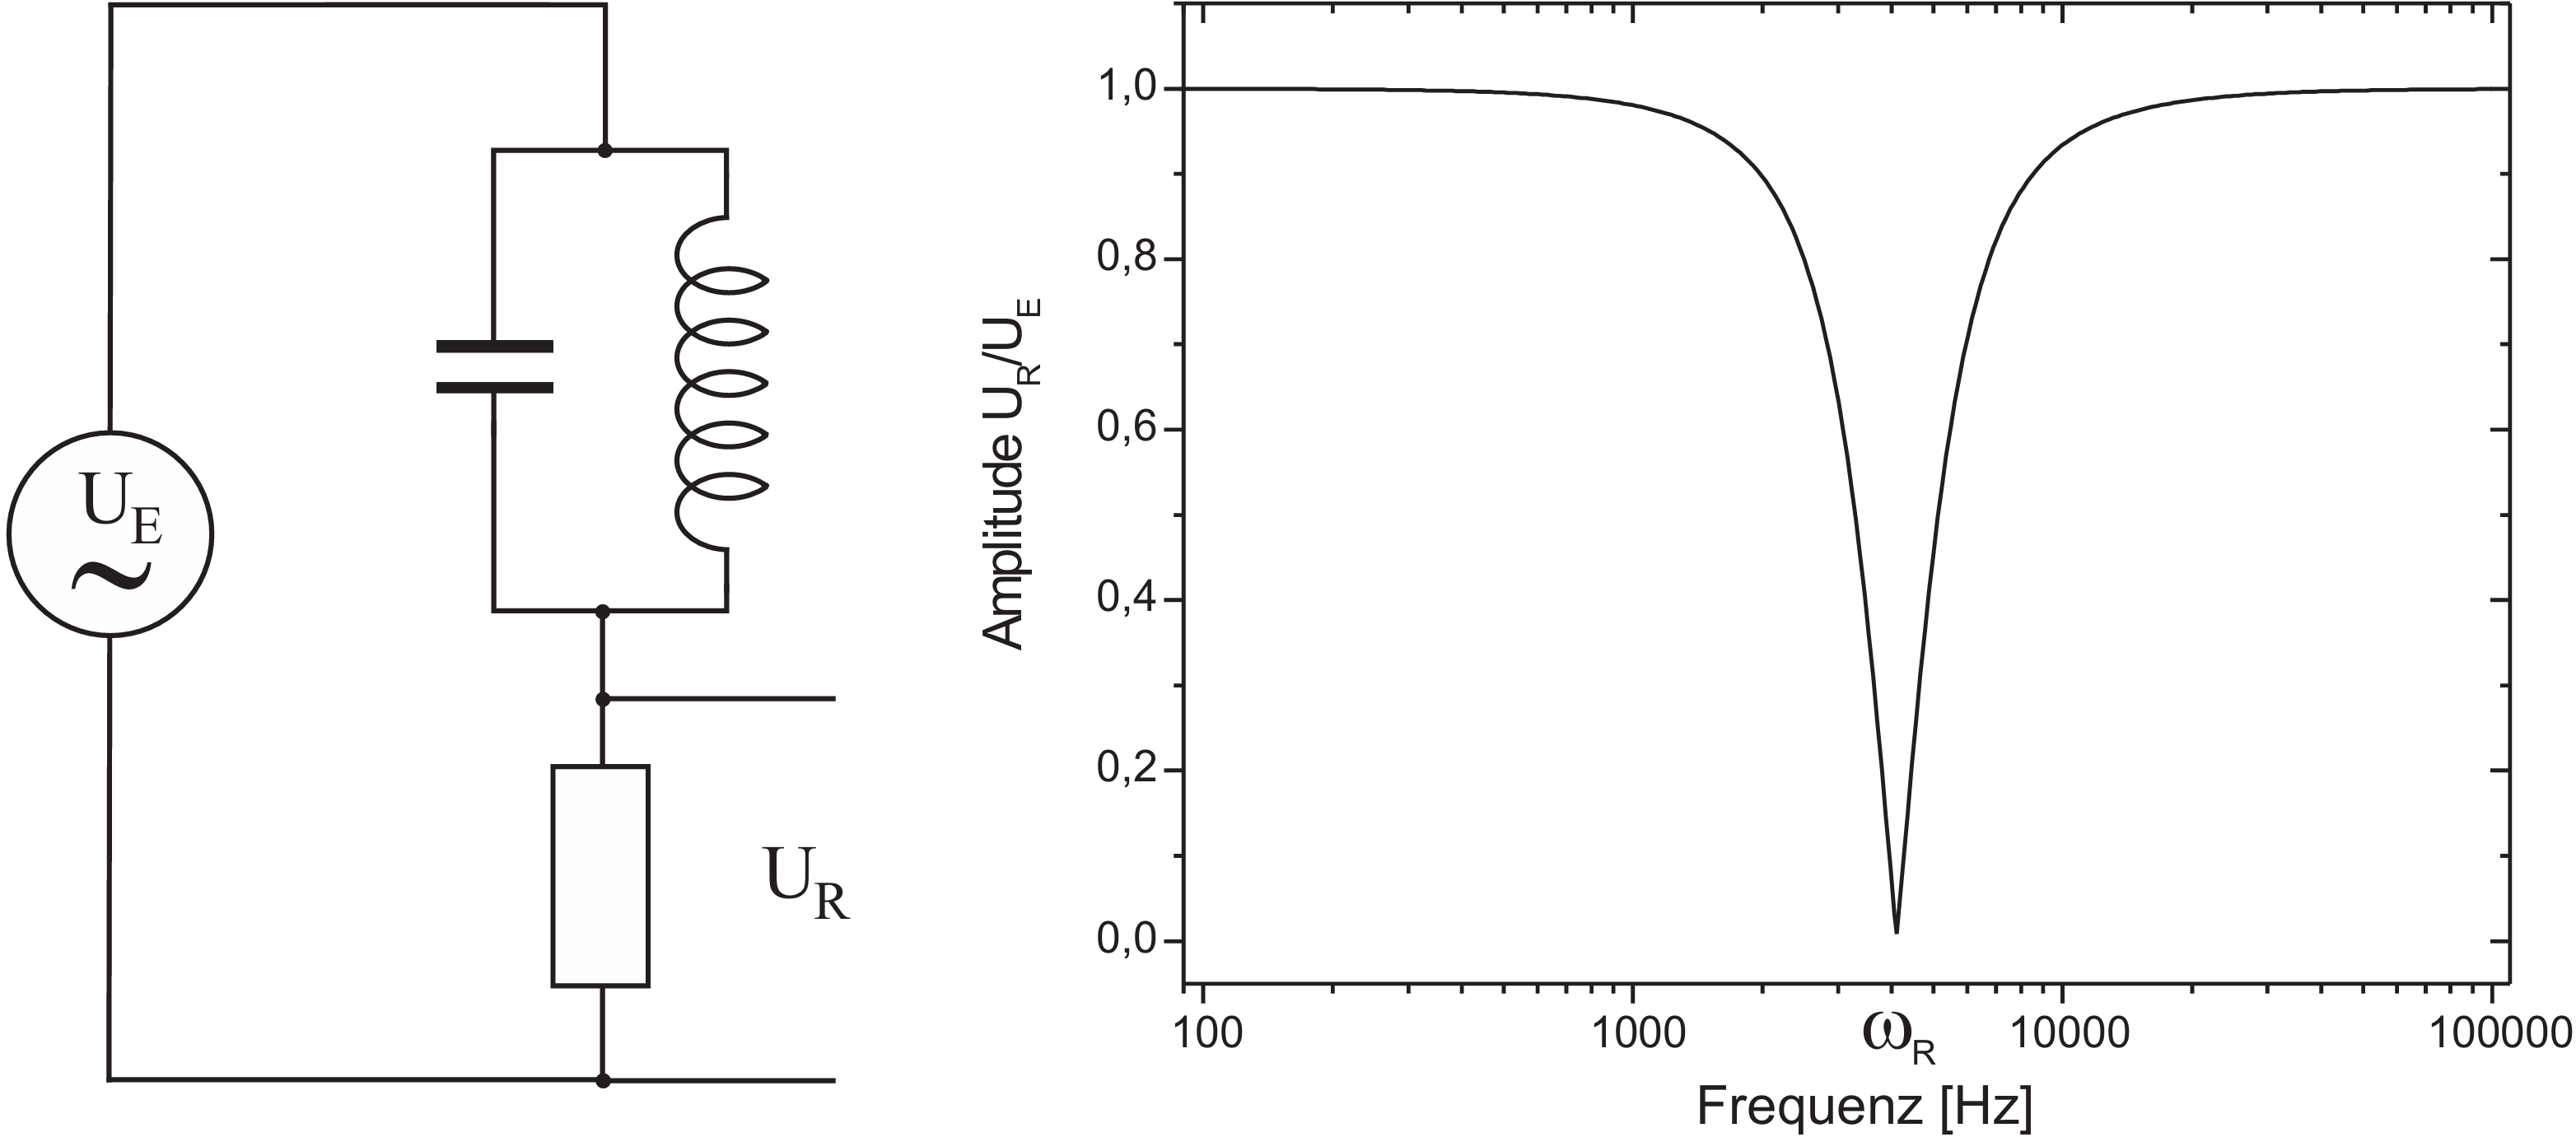
\includegraphics[width=.70\textwidth]{files/script/parallelschwingkreis.png}
  \caption{Schaltplan des Parallelschwingkreis}
  \label{fig:parallelschwingkreis}
\end{figure}

\subsubsection*{Anwendungen von LC-Gliedern: Radioempfänger}

Ein Anwendungsbereich von LC-Gliedern als Bandpassfiltern sind Radioempfänger. Bevor ein Signal empfangen werden kann, muss es jedoch zunächst gesendet werden. Radio Sender nutzen die sogenannte Modulation, um ein das niederfrequente Signal, welche Musik und Sprache enthält, im Bereich von $100 \si{\hertz}$ bis $4 \si{\kilo\hertz}$ einem höherfrequenten Signal aufzuprägen. Dies ist notwendig, da nur so eine effektive Abstrahlung des Signals durch eine Antenne möglich ist. Bei der Amplitudenmodulation wird das hochfrequente Trägersignal mit dem zu übertragenden Signal multipliziert und so dessen Amplitude entsprechend verändert. Das modulierte Signal kann dann mit einer Antenne gesendet und empfangen werden. 

Um das empfangene Signal hörbar zu machen, muss es zunächst auf den rein positiven oder rein negativen Teil der Schwingung abgeschnitten werden. Diese Demodulation ist notwendig, da das eingehende symmetrische Signal im Mittelwert verschwindet und somit keine Schwingung der Lautsprechermembran auslöst. Durch einen Kondensator kann dann, aufgrund dessen frequenzabhängiger Impedanz $Z \propto \ffrac{1}{\omega}$, das hochfrequente Trägersignal herausgefiltert werden. Dem Ganzen kann ein LC-Schwingkreis vorgeschaltet werden, um die Wahl eines Senders zu ermöglichen. Jeder Sender sendet auf einer anderen Trägerfrequenz und ohne Filterschaltung würde jede dieser Frequenzen gleichermaßen empfangen und am Lautsprecher wiedergegeben werden. Wie zuvor beschrieben, wirkt ein LC-Schwingkreis wie ein Bandpassfilter. Stimmt man nun die Resonanzfrequenz des Schwingkreises genau so ab, dass diese der Trägerfrequenz eines bestimmten Radiosenders entspricht, so kann nur dessen Signal den Filter passieren. Um Sender mit dicht beieinanderliegenden Trägerfrequenzen zu trennen, ist eine hohe Güte und geringe Bandbreite des Schwingkreises erforderlich, weshalb in alten Radioempfängern mehrere verstärkte Kreise in Reihe geschaltet wurden, um die eine steilere Durchlasskurve und bessere Trennschärfe zu gewährleisten.
\newpage
\subsection{Versuchsdurchführung}

Der Versuch umfasst insgesamt neun Versuchsteile, von welchen der erste Teil Wechselstromeigenschaften passiver Bauteile und charakteristischen Größen von RC-Filtern und RLC-Schwingkreisen und der zweite Teil mit der praktischen Anwendung von RLC-Schaltungen umfasst. Die grundlegende Schaltung, welche für nahezu alle Versuchsteile zum Einsatz kommt, ist in \abbref{fig:schaltplan_versuchsdurchfuehrung} zu sehen.

\begin{figure}[H]
  \centering
  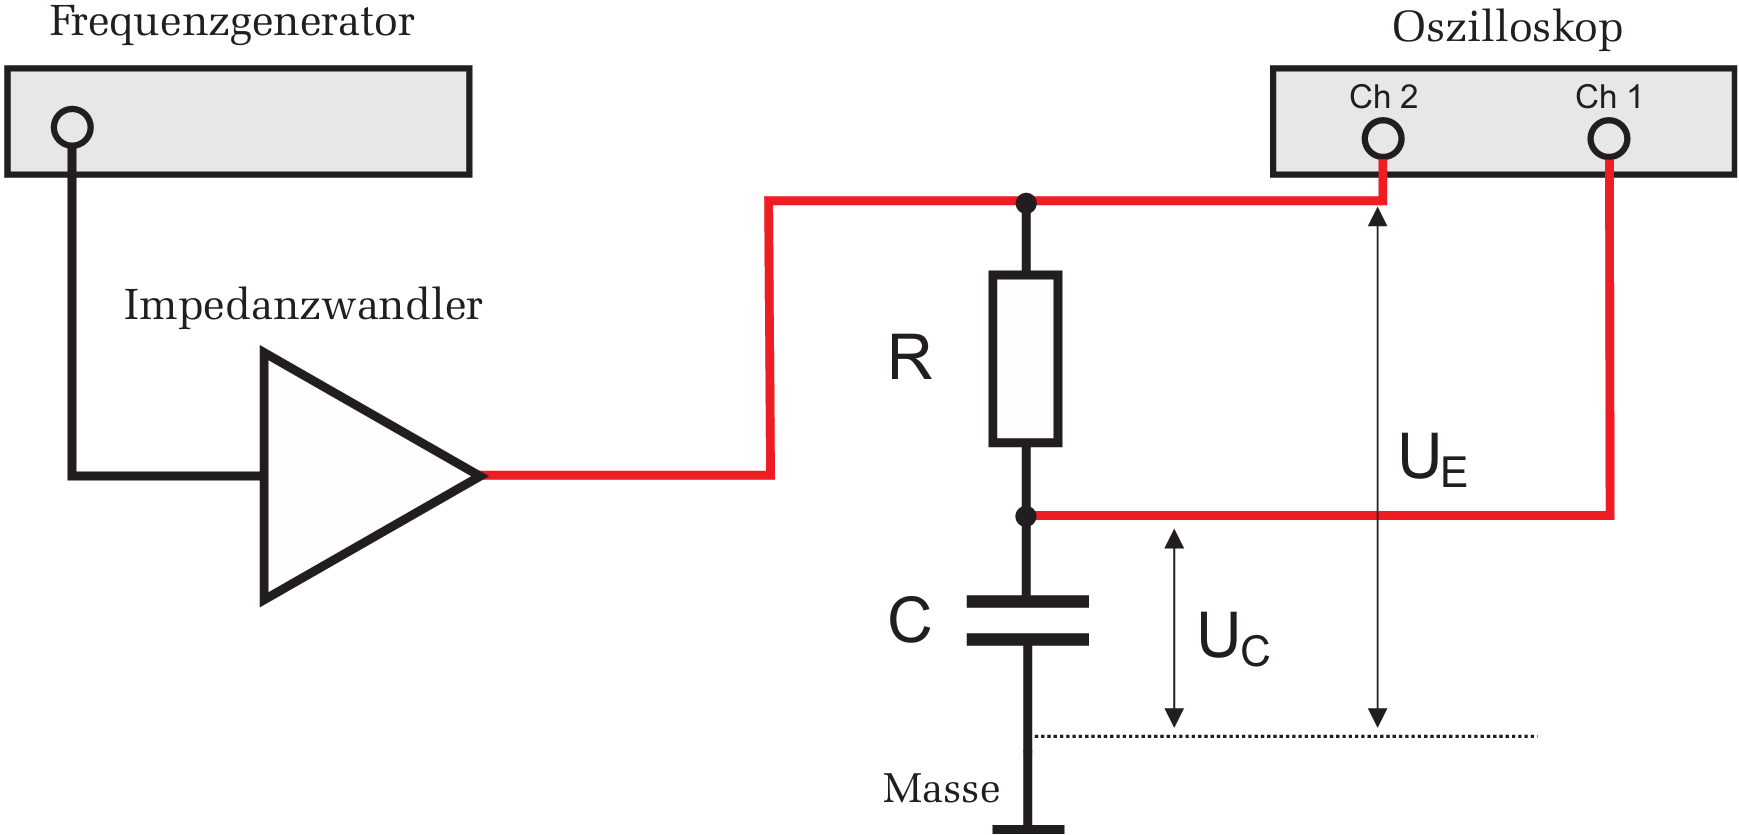
\includegraphics[width=.70\textwidth]{files/script/schaltplan_versuchsdurchfuehrung.png}
  \caption{Allgemeiner Schaltplan für die Versuchsdurchführung}
  \label{fig:schaltplan_versuchsdurchfuehrung}
\end{figure}

\textbf{Aufgabe 1: Bestimmung der Zeitkonstante eines RC-Gliedes.} Für ein Rechteckssignal, welches wir mit dem Frequenzgenerator generieren, bestimmen wir in einer RC-Schaltung für verschiedene Werte von Kapazität und Widerstand die Halbwertszeit der Kondensatorentladung. Wir vermessen die Halbwertszeit für die Werte
\begin{enumerate}
  \item $C = 470 \si{\nano\farad}$, $R = 1 \si{\kilo\ohm}$
  \item $C = 4.7 \si{\nano\farad}$, $R = 10 \si{\kilo\ohm}$
  \item $C = 47 \si{\nano\farad}$, $R = 1 \si{\kilo\ohm}$
\end{enumerate}
anhand der Spannung am Kondensator. Weiter prüfen wir durch Abnahme der Spannung am Widerstand, dass die Zeitkonstante des Stromverlaufs der des Spannungsverlaufs am Kondensator gleicht.

\textbf{Aufgabe 2: RC-Glied als Integrator und Differentiator.} In eine RC-Scahltung mit einem $47 \si{\nano\farad}$ Kondensator und einem Potentiometer ($5\si{\kilo\ohm}$) geben wir durch einen Signalgenerator verschiedenförmige Eingangssignale ein. Wir greifen die Spannung am Kondensator ab. Durch Anpassung des Wertes am Potentiometer beobachten wir die Wirkung der Schaltung als Integrator auf das jeweilige Eingangssignal. Im zweiten Teil vertauschen wir Kapazität und Widerstand, greifen die Spannung am Widerstand ab und erhalten so einen Differentiator. Mit diesem führen wir die gleichen Untersuchungen durch.

\textbf{Aufgabe 3: Frequenz- und Phasengang eines RC-Glieds.} Für eine Tief- und eine Hochpassfilterschaltung aus einem $47\si{\nano\farad}$ Kondensator und einem $1 \si{\kilo\ohm}$ Widerstand nehmen wir jeweils den Frequenzgang für einen Bereich von $100\si{\hertz}$ bis $100\si{\kilo\hertz}$ auf. Als Eingangssignal verwenden wir jeweils ein Sinussignal mit $2 \si{\volt}$ peak-to-peak. Aus dem Frequenzgang vermessen wir jeweils die Grenzfrequenz der Filterschaltung. Weiter bestimmen wir durch manuelles Messen der Phasenverschiebung zwischen Ein- und Ausgangsspannung den Phasengang des Hochpassfilters.

\textbf{Aufgabe 4: Frequenzgang eines Serienschwingkreis.} Wir erweitern den eben untersuchten RC-Schaltkreis mit der Spule $L_1$ zu einem Serienschwingkreis. Wir verwenden das gleiche Eingangssignal wie zuvor und zeichnen den Frequenzgang für einen Bereich von $1 \si{\kilo\hertz}$ bis $10 \si{\kilo\hertz}$, jeweils für die Widerstände $R = 1 \si{\kilo\ohm}$, $220 \si{\ohm}$ und $47 \si{\ohm}$ auf. Die Ausgangsspannung nehmen wir hierzu am Widerstand ab. Aus dem Frequenzgang bestimmen wir die Resonanzfrequenz $f_R$, die Bandbreite $\Delta f$, sowie die Effektivwerte der Aus- und Eingangsspannung bei der Resonanzfrequenz.

\textbf{Aufgabe 5: Resonanzüberhöhung.} Für einen Serienschwingkreis mit Kapazität $47 \si{\nano\farad}$, Widerstand $220 \si{\ohm}$ und Induktivität $L_1$ zeichnen wir den Frequenzgang jeweils einmal über jedes Bauteil auf. Aus den Maxima der Verläufe bestimmen wir die Resonanzfrequenzen.

\textbf{Aufgabe 6: Bestimmung der Dämpfungskonstante eines freien, gedämpften Schwingkreises.} Wir betrachten einen Serienschwingkreis mit Kapazität $47 \si{\nano\farad}$, Widerstand $47 \si{\ohm}$ und Induktivität $L_1$ und greifen die Ausgangsspannung über die Spule ab. Als Eingangssignal generieren wir mit dem Funktiongenerator ein Rechteckssignal, dessen Frequenz so gewählt ist, dass ein kompletter gedämpfter Schwingungsvorgang pro Ausschlag möglich ist. Um das logarithmische Dekrement bestimmen zu können, vermessen wir die Amplituden von fünf benachbarten Schwingungen. Wir ersetzen dann den Widerstand durch einen Potentiometer, um den Schwingungsvorgang abhängig von der Dämpfung beobachten zu können.

\textbf{Aufgabe 7: Parallelschwingkreis - Bandsperre.} Nun betrachten wir einen Parallelschwingkreis mit Kapazität $47 \si{\nano\farad}$, Widerstand $1 \si{\kilo\ohm}$ und Induktivität $L_1$. Wir zeichnen den Frequenzgang der Schaltung für einen Frequenzbereich von $100 \si{\hertz}$ bis $100 \si{\kilo\hertz}$ auf und bestimmen aus diesem die Resonanzfrequenz des Schwingkreises.

\textbf{Aufgabe 8: Signalformung.} In diesem Aufgabenteil verwenden wir verschiedene Filterschaltungen, um bestimmte Frequenzanteile aus einer Menge an überlagerten Signalen herauszufiltern. Mithilfe des Signalgenerators erzeugen wir ein Signal, welches aus drei überlagerten Sinussignalen unterschiedlicher Frequenz ($100 \si{\hertz}, 4 \si{\kilo\hertz}, 8 \si{\kilo\hertz}$) und Amplitude, sowie jede Menge weiterer hinzuaddierter Störsignale besteht. Mithilfe des \textit{Spectrum Analyzer} der Oszilloskopsoftware vermessen wir für jeden der folgenden verwendeten Filterschaltungen die Amplitude und Frequenz der drei stärksten Signale des Frequenzspektrums:

\begin{multicols}{2}
  \begin{enumerate}[label=\arabic*.]
    \item Ohne Filter, $R = 220 \si{\ohm}$
    \item RC- und LC-Schaltungen; Hoch-/Tiefpassfilter
    \begin{enumerate}[label=\alph*)]
      \item Hochpass, $R = 220 \si{\ohm}, C = 470 \si{\nano\farad}$
      \item Tiefpass, $R = 220 \si{\ohm}, C = 470 \si{\nano\farad}$
      \item LC-Tiefpass, $L = L_1, C = 47 \si{\nano\farad}$
    \end{enumerate}
    \item RLC-Schaltung; Bandpass-Filter
    \begin{enumerate}[label=\alph*)]
      \item $\qty|U_A|$ über Kondensator
      \begin{enumerate}
        \item $R = 1 \si{\kilo\ohm}, L = L_1, C = 47 \si{\nano\farad}$
        \item $R = 47 \si{\ohm}, L = L_1, C = 47 \si{\nano\farad}$
      \end{enumerate}
      \item $\qty|U_A|$ über Spule
      \begin{enumerate}
        \item $R = 1 \si{\kilo\ohm}, L = L_1, C = 47 \si{\nano\farad}$
        \item $R = 47 \si{\ohm}, L = L_1, C = 47 \si{\nano\farad}$
      \end{enumerate}
      \item $\qty|U_A|$ über Widerstand
      \begin{enumerate}
        \item $R = 1 \si{\kilo\ohm}, L = L_1, C = 47 \si{\nano\farad}$
        \item $R = 47 \si{\ohm}, L = L_1, C = 47 \si{\nano\farad}$
      \end{enumerate}
    \end{enumerate}
  \end{enumerate}
  \vspace*{5em}
\end{multicols}

\newpage

\textbf{Aufgabe 9: Aufbau eines einfachen AM-Empfängers.} Wir bauen aus dem Drehkondensator ($500\si{\pico\farad}$) und der Spule $L_2$ einen Parallelschwingkreis als Bandpassfilter auf. Diesen verbinden wir mit der Antennenbuchse. Ziel ist es ein über eine Sendeantenne im Raum gesendetes Sinussignal, zu empfangen und möglichst störungsfrei am Oszilloskop anzeigen. Zunächst greifen wir die Spannung direkt am Drehkondensator mit dem Oszilloskop ab und beobachten die Wirkung des Filters auf das Frequenzspektrum. Hierzu variieren wir die Kapazitäten durch den Drehkondensator und die Induktivität durch einen Eisenkern in der Spule.

Dann fügen wir in die Schaltung eine Diode zur demodulation und einen hochohmigen Kopfhörer mit ein. Mit diesem einfachen Radioempfänger versuchen wir nun, durch Anpassung des Drehkondensators das von einer Antenne im Raum entsendete Radiosignal hörbar zu machen.
